\documentclass[border=10pt]{standalone}

\usepackage{tikz}
\usepackage{tikzsymbols}
\usetikzlibrary{calc,patterns,shapes.geometric}

\def\centerarc[#1](#2)(#3:#4:#5){\draw[#1] ($(#2)+({#5*cos(#3)},{#5*sin(#3)})$) arc (#3:#4:#5);}

\begin{document}
	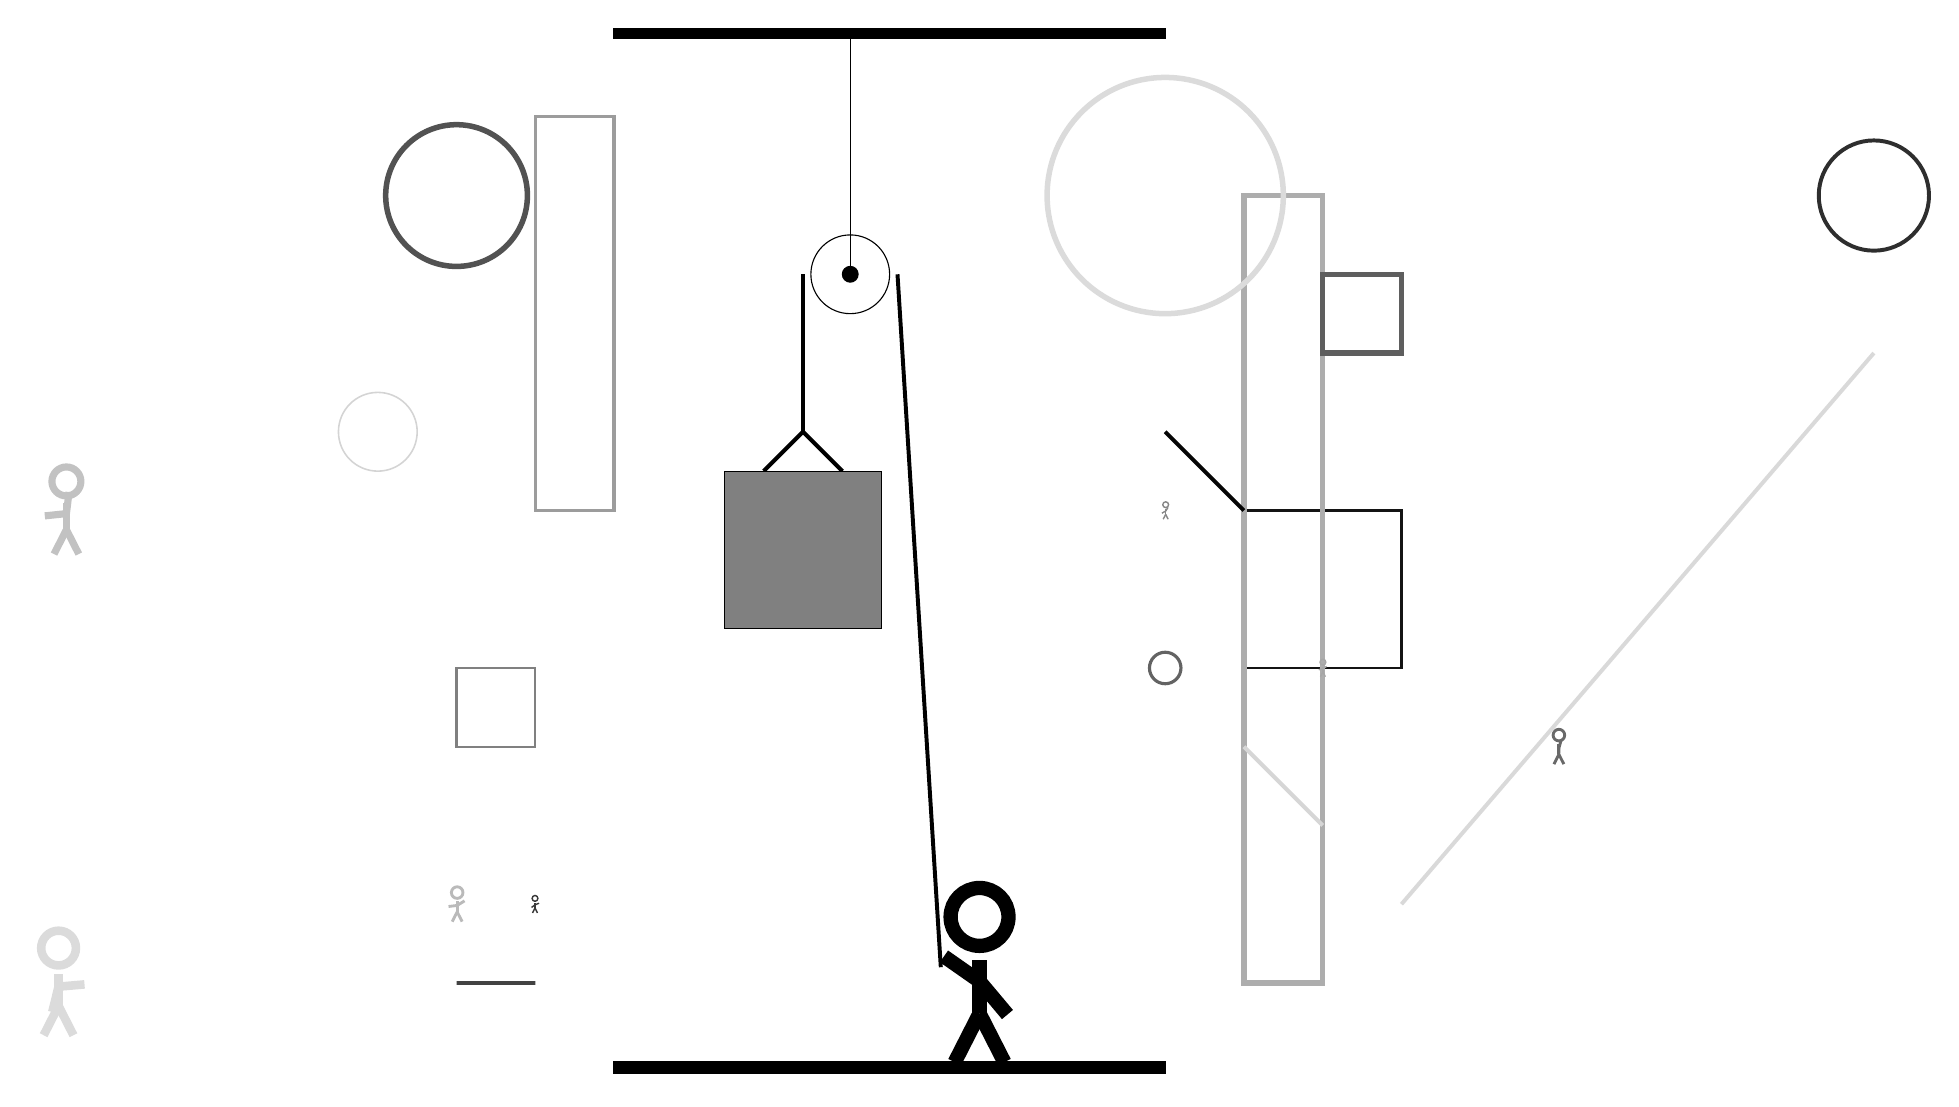
\begin{tikzpicture}
		%%%%% START %%%%%
		
		\draw[fill=black] (-2, 10) rectangle (5, 10.125);
		
		\draw (1, 7) circle (0.5);
		\draw[fill=black] (1, 7) circle (0.1);
		\draw (1, 10) -- (1, 7);
		
		\node[line width=0.5mm, color=black!78] at (-3, -1) {\Strichmaxerl[1][37][22]};
		
		\draw [line width=0.5mm, color=black!82](14, 8) circle (0.7);
		\node[line width=0.5mm, color=black!14] at (-9, -2) {\Strichmaxerl[6][76][5]};
		\draw[line width=0.3mm, color=black!92] (6, 4) rectangle (8, 2);
		\draw [line width=0.2mm, color=black!17](-5, 5) circle (0.5);
		\draw[line width=0.7mm, color=black!32] (6, -2) rectangle (7, 8);
		\draw[line width=0.3mm, color=black!50] (-3, 2) rectangle (-4, 1);
		
		\node[line width=0.3mm, color=black!47] at (5, 4) {\Strichmaxerl[1][28][58]};
		\node[line width=0.7mm, color=black!35] at (7, 2) {\Strichmaxerl[1][15][31]};
		
		\draw [line width=0.4mm, color=black!61](5, 2) circle (0.2);
		\draw[line width=0.5mm, color=black!16](6, 1) -- (7, 0);
		\draw[line width=0.6mm, color=black!74] (-4, -2) rectangle (-3, -2);
		\node[line width=0.3mm, color=black!27] at (-4, -1) {\Strichmaxerl[2][7][32]};
		
		\draw[line width=0.7mm, color=black!63] (7, 6) rectangle (8, 7);
		\node[line width=0.5mm, color=black!59] at (10, 1) {\Strichmaxerl[2][89][74]};
		\draw[line width=0.4mm, color=black!39] (-2, 9) rectangle (-3, 4);
		
		\draw [line width=0.7mm, color=black!68](-4, 8) circle (0.9);
		
		\node[line width=0.5mm, color=black!24] at (-9, 4) {\Strichmaxerl[5][6][83]};
		\draw[line width=0.5mm, color=black!15](8, -1) -- (14, 6);
		
		\draw[line width=0.5mm, color=black!98](6, 4) -- (5, 5);
		\draw [line width=0.7mm, color=black!14](5, 8) circle (1.5);
		
		
		\draw[line width=0.5mm] (-0.1, 4.5) -- (0.4, 5.0) -- (0.9, 4.5);
		\draw[fill=black!50] (-0.6, 4.5) rectangle (1.4, 2.5);
		
		\draw[line width=0.5mm] (0.4, 7) -- (0.4, 5.0);
		\centerarc[line width=0.5mm](1, 7)(0:180:0.6);
		\draw[line width=0.5mm](1.6, 7) -- (2.15, -1.8);
		
		\node at (2.6, -1.9) {\Strichmaxerl[10][-35][-50]};
		
		\draw[fill=black] (-2, -3) rectangle (5, -3.15);
		
		%%%%% END %%%%%
	\end{tikzpicture}
\end{document}